%%%%%%%%%%%%%%%%%%%
% EVALUATION INTRO
%%%%%%%%%%%%%%%%%%%
\begin{frame}{Problem}
\begin{center}
How do you evaluate open domain triples?
\end{center}
\end{frame}

\def\title{Extrinsic Evaluation: Knowledge Base Population}
\begin{frame}[noframenumbering]{\title}
\begin{center}
\begin{tabular}{cccc}
  \begin{tabular}{c}
    \h{Unstructured Text} \\
    \\
    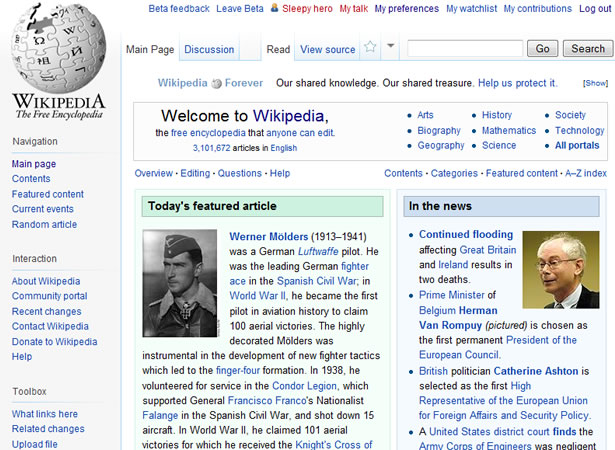
\includegraphics[width=2cm]{../img/wiki.jpg} \\
    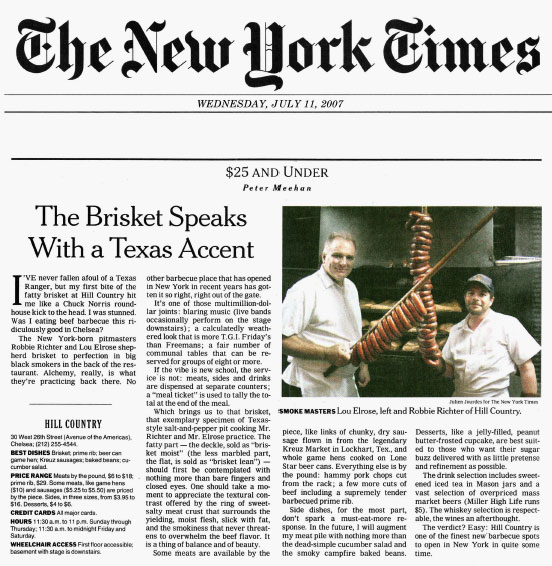
\includegraphics[width=2cm]{../img/nyt.jpg} \\
    
\includegraphics[width=2cm]{../img/blog.jpg}
  \end{tabular} &

  \Huge{$\Rightarrow$} &
  
  \begin{tabular}{c}
  \h{Structured Knowledge Base} \\
  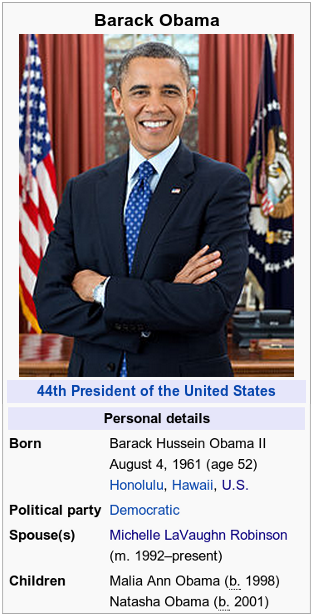
\includegraphics[width=2.75cm]{../img/obama-infobox.png}
  \end{tabular}
\end{tabular}
\end{center}
\end{frame}

\begin{frame}[noframenumbering]{\title}
\hh{Relation Extraction Task:}
\begin{itemize}
  \item Fixed schema of 41 relations.
  \item Precision: answers marked correct by humans.
  \item Recall: answers returned by any team (including LDC annotators).
\end{itemize}
\pause
\vspace{1em}

\hh{Comparison:} \textit{Open Information Extraction to KBP Relations in 3 Hours}.
  (Soderland et. al)

\begin{center}
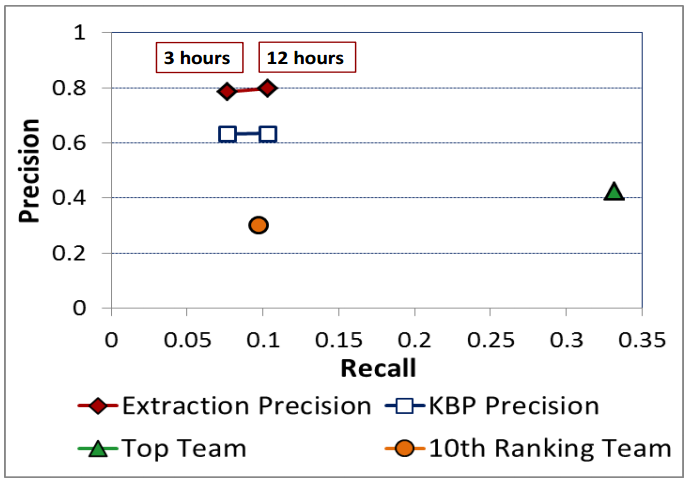
\includegraphics[scale=0.20]{../img/uw-openie.png} \\
\end{center}
\end{frame}

%%%%%%%%%%%%%%%%%%%
% RELATION MAPPING
%%%%%%%%%%%%%%%%%%%
\def\title{Prerequisite Task: Open IE $\rightarrow$ KBP Relations}
\begin{frame}{\title}
\begin{enumerate}
  \item Hand-coded mapping. \\
        (Same as UW; both over 1-2 weeks)
        \pause
        \vspace{1em}

  \item Learned relation mapping.
  \begin{itemize}
    \item For each type signature $t_1, t_2$;
    \item For an open IE relation $r_o$ and KBP relation $r_k$;
    \pause
    \item Compute:
      \begin{center}
        $
        p(r_k, r_o \mid t_1, t_2) = \frac{
          \textrm{count}(r_k, r_o,  t_1, t_2)
        }{
          \sum_{r_k', r_o'}\textrm{count}(r_k', r_o', t_1, t_2)
        }
        $.
      \end{center}
    \pause
    \item Rank by PMI$^2(r_o, r_k \mid t_1, t_2)$:
      \begin{center}
        $
        \textrm{PMI}^2(r_k, r_o \mid t_1, t_2) = \log \left( \frac{p(r_k, r_o \mid t_1, t_2)^2}{p(r_k \mid t_1, t_2) \cdot p(r_o \mid t_1, t_2)} \right)
        $.
      \end{center}
  \end{itemize}
\end{enumerate}
\end{frame}

\begin{frame}[noframenumbering]{\title}
\begin{center}
\begin{tabular}{l:lc}
  \textbf{KBP Relation} & \textbf{Open IE Relation} & \textbf{PMI$^2$}\\
  \hline
  \small{\rel{Per:Date\_Of\_Birth}}    & \ww{be bear on} & 1.83       \\
                                       & \ww{bear on} & 1.28          \\
  \small{\rel{Per:Date\_Of\_Death}}   & \ww{die on} & 0.70  \\
                                      & \ww{be assassinate on} & 0.65  \\
  \small{\rel{Per:LOC\_Of\_Birth}}     & \ww{be bear in} & 1.21        \\
  \small{\rel{Per:LOC\_Of\_Death}}     & \ww{\darkred{*elect president of}} & 2.89                \\
  \small{\rel{Per:Religion}}          & \ww{speak about} & 0.67   \\
                                      & \ww{popular for} & 0.60   \\
  \small{\rel{Per:Parents}}            & \ww{daughter of}     & 0.54          \\
                                      & \ww{son of} & 1.52          \\
  \small{\rel{Per:LOC\_Residence}}     & \ww{of} & 1.48       \\
                                       & \ww{\darkred{*independent from}} & 1.18    \\
\end{tabular}
\end{center}
\end{frame}

%%%%%%%%%%%%%%%%%%%
% RESULTS
%%%%%%%%%%%%%%%%%%%
\def\title{Results}
\begin{frame}{\title}
\hh{TAC-KBP 2013 Slot Filling Challenge:}
\begin{itemize}
  \item End-to-end task -- includes IR + consistency.
\item \textbf{Precision:} facts LDC evaluators judged as correct. \\
      \textbf{Recall:} facts other teams (including LDC annotators) also found.
\end{itemize}
\vspace{0.25cm}

\def\bell{\raisebox{-2.5mm}{
\includegraphics[height=5mm]{../img/bell.png}}}
\def\whistle{\raisebox{-2.5mm}{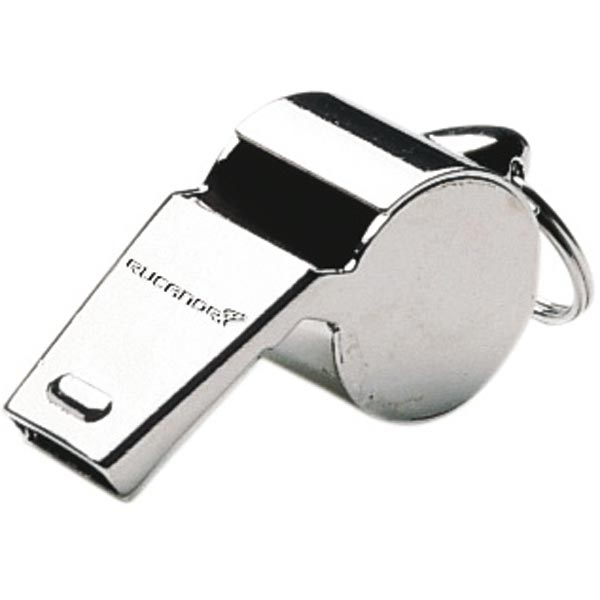
\includegraphics[height=5mm]{../img/whistle.jpg}}}
\begin{center}
\begin{tabular}{lrrr}
\hline
\textbf{System}                & \multicolumn{1}{c}{\textbf{P}}    
                               & \multicolumn{1}{c}{\textbf{R}}    
                               & \multicolumn{1}{c}{\textbf{F$_1$}} \\
\hline
UW Submission                   & 69.8          & 11.4          & 19.6 \\
Ollie                           & 57.7          & 11.8          & 19.6 \\
\pause
\darkblue{Our System}           & \darkblue{61.9} & \darkblue{13.9} & \darkblue{22.7} \\
\hline
\pause
Median Team                     &               &               & 18.6 \\
\darkblue{Our System} + \bell\ + \whistle  & \darkblue{58.6} & \darkblue{18.6} & \darkblue{28.3} \\
Top Team                        & 45.7          & 35.8          & 40.2 \\
\hline
\end{tabular}
\end{center}
\end{frame}
